% experiment

\section{Experiments}
\subsection{Experimental setup}
Our project will be divided into three parts: a 2-bit counter to track the re-reference Interval Prediction Value(RRPV); The Signature HIstory Counter Table(SHCT) of saturating counters to learn the re-reference behavior of a signature and bypassing topology.
\begin{itemize}
    \item \(RRPV\): 2-bit counter. As shown in fig. \ref{fig.RRPV}, upon a hit to the line, the RRPV is reset to 0. In the event of a miss, the victim is identified by commencing the search from way 0 and locating the first line in the set with an RRPV of 3. If no such line is found, the RRPV of all lines in the set is incremented, and the search is conducted once more. The RRIP can insert the line with either a high-priority position (RRPV=2) or a low-priority position (RRPV=3). The selection of the insertion position can be determined either statically for all references, as in the case of SRRIP, or dynamically at runtime, as with DRRIP. 
    
\begin{figure}[htbp]
\centering
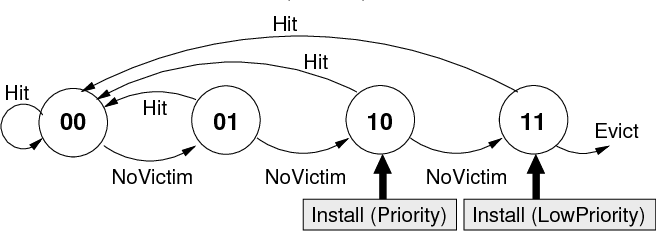
\includegraphics[width=0.5\textwidth]{figs/RRPV.png}
\caption{Re-reference Interval Prediction.}
\label{fig.RRPV}
\end{figure}

    \item \(SHCT\): 3-bit counter, as shown in fig. \ref{fig.SHCT}, SHIP necessitates the storage of two additional fields with each cache line: the signature (Program Counter, or PC, has been chosen for this project) and a single-bit to monitor the outcome of the cache insertion. The outcome bit, initially set to zero, is assigned a value of one only if the cache line is re-referenced. SHIP also employs a Signature History Counter Table (SHCT) of saturating counters, indexed by the signature associated with the cache line. Upon a hit to a cache line, SHIP increments the SHCT entry indexed by the signature stored with the cache line. Conversely, when a line is evicted from the cache without being re-referenced since insertion, SHIP decrements the SHCT entry indexed by the PC signature associated with the evicted cache line.
    
\begin{figure}[htbp]
\centering
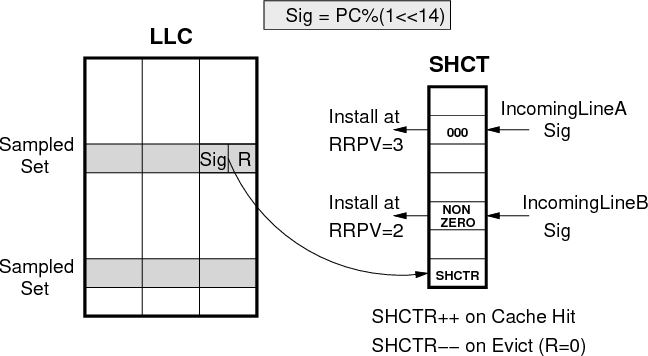
\includegraphics[width=0.5\textwidth]{figs/SHCT.png}
\caption{Signature History Counter Table.}
\label{fig.SHCT}
\end{figure}
    \item \(Bypassing\): The objective is to safeguard valuable data. Nevertheless, when the working set of data exceeds the cache size, resulting in a high rate of cache misses and the incessant eviction and loading of data, such as in the case of cache thrashing, bypassing becomes unfeasible. As a result, an approach is explored to quantify the number of valuable data elements in a specific manner and subsequently determine whether or not to execute bypassing.
\end{itemize}


\subsection{Discussion}
As demonstrated in Table. \ref{table.util}, the proposed policy outperforms SHIP++ in the current evaluation.
\begin{table}[htbp]
\caption{Result Summary}
\begin{center}
\begin{tabular}{|c|c|}
\hline
\textbf{Policy}&\textbf{GeoMean compared with LRU}\\
\hline
SHiP++(16K/3-bit SHCT) & 1.0268\\
\hline
Simple Bypass when SHCT = 0 & 1.0181\\
\hline
Bypass when SHCT = 0 \\and at least 14 recently used ways & 1.028\\
\hline
Same policy but 16k/2-bit SHCT &   1.0284\\
\hline
Same policy but 4k/3-bit SHCT  &   1.0282\\
\hline
Same policy but 4k/2-bit SHCT  &   1.0281\\
\hline
\end{tabular}
\label{table.util}
\end{center}
\end{table}
Also, there are many other ways to improve the utilization of the SHCT table.
\begin{itemize}
    \item \(Adaptive sizing\): Dynamically adjusting the size of the SHCT table based on the workload characteristics can help in maintaining an optimal table size, reducing hardware storage requirements without sacrificing performance.
    \item \(Intelligent initialization\): Instead of initializing all SHCT entries with the same value, consider using a smarter initialization strategy based on prior knowledge of the workload or by learning during an initial warm-up phase. This can help improve prediction accuracy and reduce the time it takes for the table to become useful.
    \item \(Aging mechanisms\): Implement an aging mechanism to periodically decrement or reset the counters in the SHCT table. This prevents counters from becoming saturated and allows the table to adapt to changes in access patterns over time.
    \item \(Multi-level SHCT\): Introduce a hierarchical SHCT structure with multiple levels to capture and predict different levels of re-reference intervals. This can provide more granular control over cache replacement decisions and improve prediction accuracy.
    \item \(Signature refinement\): Enhance the signature generation process to better differentiate between different data elements and their access patterns. This could include incorporating additional information, such as memory address bits or instruction-level information, to create more distinct and meaningful signatures.
    \item \(Hybrid approaches\): Combine SHCT with other cache replacement policies or prediction techniques to leverage the strengths of different approaches and improve overall cache performance.
\end{itemize}